\documentclass[crop=false]{standalone}
%\documentclass{standalone}
\usepackage{tikz} % To generate the plot from csv
\usepackage{pgfplots}
\usepackage{graphicx}
\usepackage{booktabs}
\usepackage{subfig}
\usepackage{float}
\usepackage[section]{placeins} % getting figures below sections
\usepackage{blindtext}
\usepackage{siunitx}
\usepgfplotslibrary{units} % Allows to enter the units nicely
\usetikzlibrary{external} %https://tex.stackexchange.com/questions/1460/script-to-automate-externalizing-tikz-graphics
\tikzexternalize[prefix=savedfigures/]

\pgfplotsset{compat=newest} % Allows to place the legend below plot
\usepackage{pgfplotstable}
\usepgfplotslibrary{statistics}

% #################### Function definition for box plots read table ##################\
\makeatletter
\pgfplotsset{
	boxplot prepared from table/.code={
		\def\tikz@plot@handler{\pgfplotsplothandlerboxplotprepared}%
		\pgfplotsset{
			/pgfplots/boxplot prepared from table/.cd,
			#1,
		}
	},
	/pgfplots/boxplot prepared from table/.cd,
	table/.code={\pgfplotstablecopy{#1}\to\boxplot@datatable},
	row/.initial=0,
	make style readable from table/.style={
		#1/.code={
			\pgfplotstablegetelem{\pgfkeysvalueof{/pgfplots/boxplot prepared from table/row}}{##1}\of\boxplot@datatable
			\pgfplotsset{boxplot/#1/.expand once={\pgfplotsretval}}
		}
	},
	make style readable from table=lower whisker,
	make style readable from table=upper whisker,
	make style readable from table=lower quartile,
	make style readable from table=upper quartile,
	make style readable from table=median,
	make style readable from table=average,
	make style readable from table=lower notch,
	make style readable from table=upper notch
}
\makeatother
\begin{document}
\pgfkeys{/pgf/number format/.cd,1000 sep={\,}}

\section{33 2 Mumford0 SA ALL param 20210818 113747}

% ######################## UTRP SA Cooling rate ######################## 
\begin{figure} 
\centering 
\tikzsetnextfilename{UTRP_DBMOSA_BP_cooling_rate} 
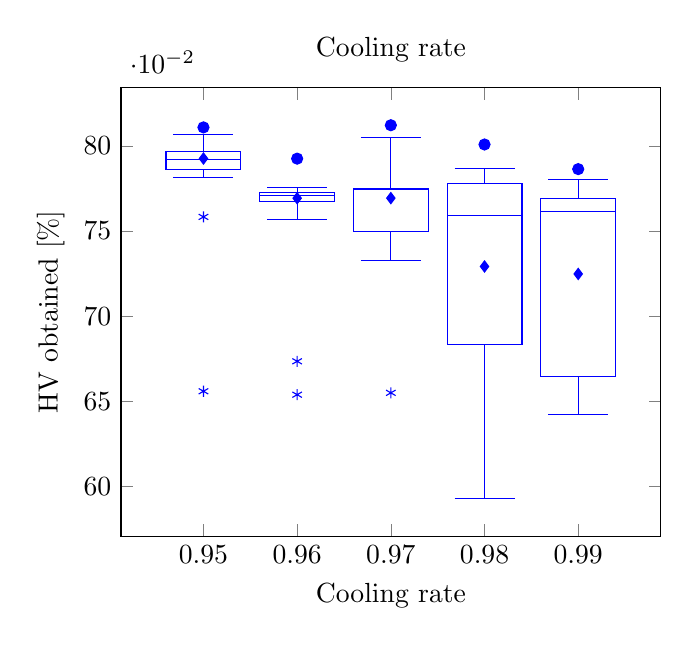
\begin{tikzpicture} 
\begin{axis}[ 
title={Cooling rate}, 
boxplot/draw direction=y, 
xtick={1,2,3,4,5}, 
xticklabels={0.95,0.96,0.97,0.98,0.99}, 
x tick label style={rotate=0, align=center}, 
xlabel={Cooling rate}, 
% y tick label style={/pgf/number format/.cd,fixed,precision=3, zerofill}, 
scaled y ticks={base 10:2}, 
ylabel={HV obtained [\%]}, 
] 

% ############## Cooling_rate=0.95 ################## 
\addplot[boxplot, mark=asterisk, 
boxplot prepared={ 
lower whisker=0.78141, 
upper whisker=0.80646, 
lower quartile=0.78601, 
upper quartile=0.79696, 
median=0.79188, 
average=0.79257}, 
color = blue, solid, area legend] 
coordinates {
(1,0.65595)
(1,0.75831)}; 
\addplot[only marks,mark=*,color = blue]coordinates{(1,0.81086)}; 

% ############## Cooling_rate=0.96 ################## 
\addplot[boxplot, mark=asterisk, 
boxplot prepared={ 
lower whisker=0.75684, 
upper whisker=0.77543, 
lower quartile=0.76718, 
upper quartile=0.77278, 
median=0.77088, 
average=0.7693}, 
color = blue, solid, area legend] 
coordinates {
(2,0.65394)
(2,0.67354)}; 
\addplot[only marks,mark=*,color = blue]coordinates{(2,0.79251)}; 

% ############## Cooling_rate=0.97 ################## 
\addplot[boxplot, mark=asterisk, 
boxplot prepared={ 
lower whisker=0.73278, 
upper whisker=0.80499, 
lower quartile=0.74972, 
upper quartile=0.77505, 
median=0.77434, 
average=0.76931}, 
color = blue, solid, area legend] 
coordinates {
(3,0.65502)}; 
\addplot[only marks,mark=*,color = blue]coordinates{(3,0.81212)}; 

% ############## Cooling_rate=0.98 ################## 
\addplot[boxplot, mark=asterisk, 
boxplot prepared={ 
lower whisker=0.5928, 
upper whisker=0.78694, 
lower quartile=0.68352, 
upper quartile=0.77814, 
median=0.75899, 
average=0.7292}, 
color = blue, solid, area legend] 
coordinates {}; 
\addplot[only marks,mark=*,color = blue]coordinates{(4,0.80082)}; 

% ############## Cooling_rate=0.99 ################## 
\addplot[boxplot, mark=asterisk, 
boxplot prepared={ 
lower whisker=0.64236, 
upper whisker=0.7803, 
lower quartile=0.66453, 
upper quartile=0.76888, 
median=0.76172, 
average=0.72483}, 
color = blue, solid, area legend] 
coordinates {}; 
\addplot[only marks,mark=*,color = blue]coordinates{(5,0.78636)}; 

\end{axis}
\end{tikzpicture}
\end{figure} 

% ######################## UTRP SA Maximum attempts ######################## 
\begin{figure} 
\centering 
\tikzsetnextfilename{UTRP_DBMOSA_BP_max_attempts} 
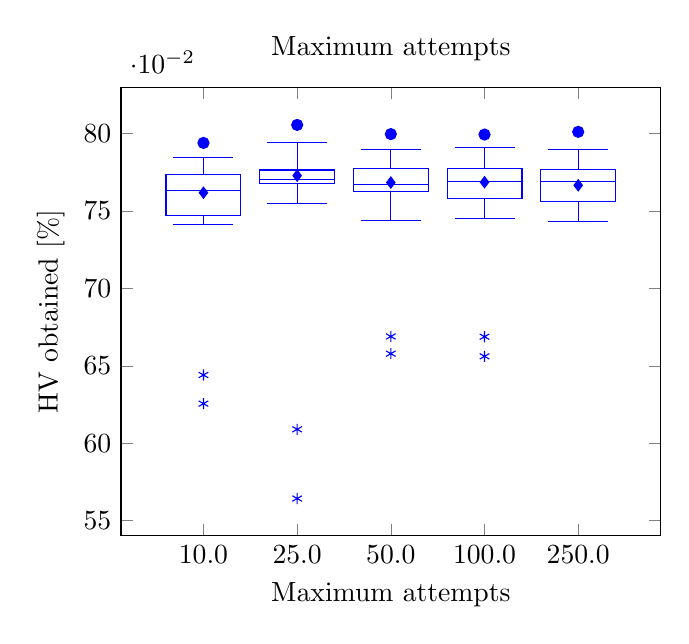
\begin{tikzpicture} 
\begin{axis}[ 
title={Maximum attempts}, 
boxplot/draw direction=y, 
xtick={1,2,3,4,5}, 
xticklabels={10.0,25.0,50.0,100.0,250.0}, 
x tick label style={rotate=0, align=center}, 
xlabel={Maximum attempts}, 
% y tick label style={/pgf/number format/.cd,fixed,precision=3, zerofill}, 
scaled y ticks={base 10:2}, 
ylabel={HV obtained [\%]}, 
] 

% ############## max_attempts=10.0 ################## 
\addplot[boxplot, mark=asterisk, 
boxplot prepared={ 
lower whisker=0.74137, 
upper whisker=0.78435, 
lower quartile=0.7472, 
upper quartile=0.77365, 
median=0.76318, 
average=0.76169}, 
color = blue, solid, area legend] 
coordinates {
(1,0.62557)
(1,0.64406)}; 
\addplot[only marks,mark=*,color = blue]coordinates{(1,0.79384)}; 

% ############## max_attempts=25.0 ################## 
\addplot[boxplot, mark=asterisk, 
boxplot prepared={ 
lower whisker=0.75472, 
upper whisker=0.79435, 
lower quartile=0.76775, 
upper quartile=0.77634, 
median=0.77025, 
average=0.77271}, 
color = blue, solid, area legend] 
coordinates {
(2,0.56433)
(2,0.60899)}; 
\addplot[only marks,mark=*,color = blue]coordinates{(2,0.80544)}; 

% ############## max_attempts=50.0 ################## 
\addplot[boxplot, mark=asterisk, 
boxplot prepared={ 
lower whisker=0.74363, 
upper whisker=0.7895, 
lower quartile=0.76242, 
upper quartile=0.77713, 
median=0.76692, 
average=0.76827}, 
color = blue, solid, area legend] 
coordinates {
(3,0.6689)
(3,0.65783)}; 
\addplot[only marks,mark=*,color = blue]coordinates{(3,0.79952)}; 

% ############## max_attempts=100.0 ################## 
\addplot[boxplot, mark=asterisk, 
boxplot prepared={ 
lower whisker=0.74483, 
upper whisker=0.79116, 
lower quartile=0.75785, 
upper quartile=0.77741, 
median=0.76878, 
average=0.76849}, 
color = blue, solid, area legend] 
coordinates {
(4,0.65609)
(4,0.66875)}; 
\addplot[only marks,mark=*,color = blue]coordinates{(4,0.79922)}; 

% ############## max_attempts=250.0 ################## 
\addplot[boxplot, mark=asterisk, 
boxplot prepared={ 
lower whisker=0.74303, 
upper whisker=0.78979, 
lower quartile=0.75601, 
upper quartile=0.77646, 
median=0.76879, 
average=0.76648}, 
color = blue, solid, area legend] 
coordinates {}; 
\addplot[only marks,mark=*,color = blue]coordinates{(5,0.80098)}; 

\end{axis}
\end{tikzpicture}
\end{figure} 

% ######################## UTRP SA Max iterations per epoch ######################## 
\begin{figure} 
\centering 
\tikzsetnextfilename{UTRP_DBMOSA_BP_max_iterations_per_epoch} 
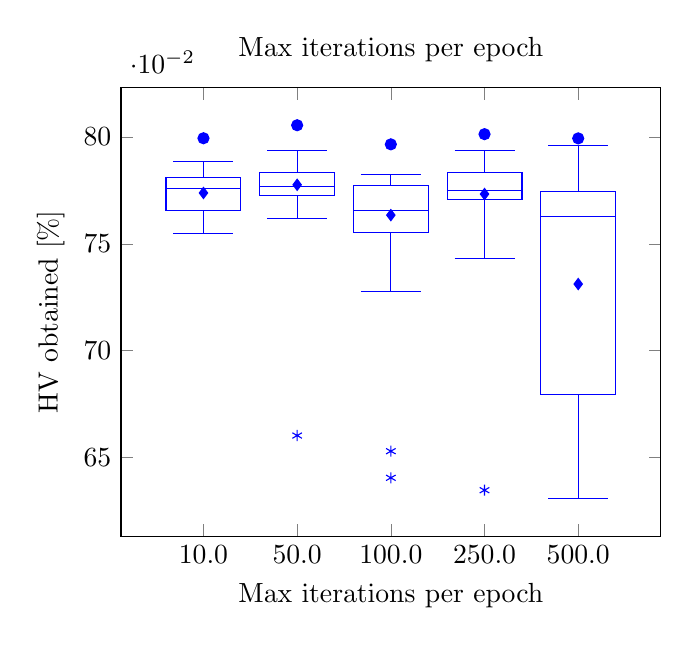
\begin{tikzpicture} 
\begin{axis}[ 
title={Max iterations per epoch}, 
boxplot/draw direction=y, 
xtick={1,2,3,4,5}, 
xticklabels={10.0,50.0,100.0,250.0,500.0}, 
x tick label style={rotate=0, align=center}, 
xlabel={Max iterations per epoch}, 
% y tick label style={/pgf/number format/.cd,fixed,precision=3, zerofill}, 
scaled y ticks={base 10:2}, 
ylabel={HV obtained [\%]}, 
] 

% ############## max_iterations_t=10.0 ################## 
\addplot[boxplot, mark=asterisk, 
boxplot prepared={ 
lower whisker=0.75499, 
upper whisker=0.78826, 
lower quartile=0.76571, 
upper quartile=0.78101, 
median=0.77587, 
average=0.77374}, 
color = blue, solid, area legend] 
coordinates {}; 
\addplot[only marks,mark=*,color = blue]coordinates{(1,0.79932)}; 

% ############## max_iterations_t=50.0 ################## 
\addplot[boxplot, mark=asterisk, 
boxplot prepared={ 
lower whisker=0.76194, 
upper whisker=0.7937, 
lower quartile=0.77251, 
upper quartile=0.78317, 
median=0.77679, 
average=0.77756}, 
color = blue, solid, area legend] 
coordinates {
(2,0.66039)}; 
\addplot[only marks,mark=*,color = blue]coordinates{(2,0.8054)}; 

% ############## max_iterations_t=100.0 ################## 
\addplot[boxplot, mark=asterisk, 
boxplot prepared={ 
lower whisker=0.72786, 
upper whisker=0.78239, 
lower quartile=0.75514, 
upper quartile=0.77716, 
median=0.76558, 
average=0.76339}, 
color = blue, solid, area legend] 
coordinates {
(3,0.65307)
(3,0.64063)}; 
\addplot[only marks,mark=*,color = blue]coordinates{(3,0.79647)}; 

% ############## max_iterations_t=250.0 ################## 
\addplot[boxplot, mark=asterisk, 
boxplot prepared={ 
lower whisker=0.74323, 
upper whisker=0.79352, 
lower quartile=0.77058, 
upper quartile=0.78334, 
median=0.7747, 
average=0.77323}, 
color = blue, solid, area legend] 
coordinates {
(4,0.63484)}; 
\addplot[only marks,mark=*,color = blue]coordinates{(4,0.80123)}; 

% ############## max_iterations_t=500.0 ################## 
\addplot[boxplot, mark=asterisk, 
boxplot prepared={ 
lower whisker=0.63081, 
upper whisker=0.79582, 
lower quartile=0.67967, 
upper quartile=0.7744, 
median=0.76276, 
average=0.73117}, 
color = blue, solid, area legend] 
coordinates {}; 
\addplot[only marks,mark=*,color = blue]coordinates{(5,0.79926)}; 

\end{axis}
\end{tikzpicture}
\end{figure} 

% ######################## UTRP SA Maximum poor epochs ######################## 
\begin{figure} 
\centering 
\tikzsetnextfilename{UTRP_DBMOSA_BP_max_poor_epochs} 
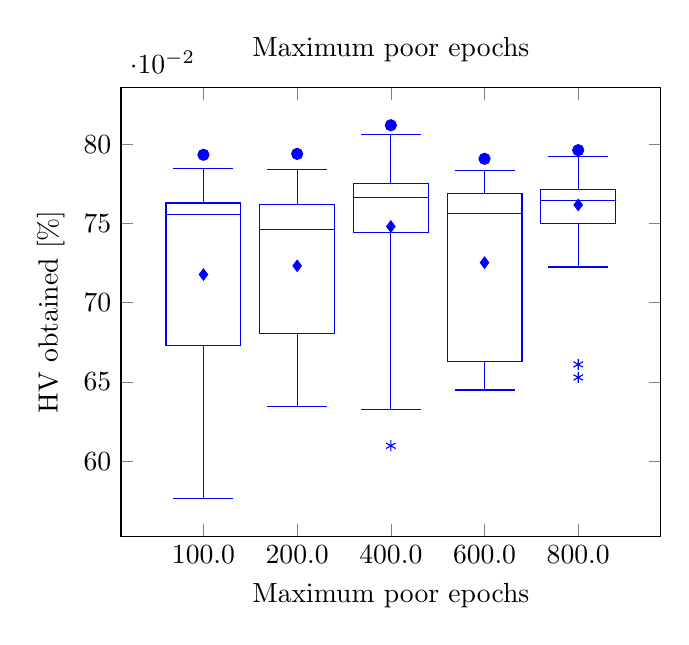
\begin{tikzpicture} 
\begin{axis}[ 
title={Maximum poor epochs}, 
boxplot/draw direction=y, 
xtick={1,2,3,4,5}, 
xticklabels={100.0,200.0,400.0,600.0,800.0}, 
x tick label style={rotate=0, align=center}, 
xlabel={Maximum poor epochs}, 
% y tick label style={/pgf/number format/.cd,fixed,precision=3, zerofill}, 
scaled y ticks={base 10:2}, 
ylabel={HV obtained [\%]}, 
] 

% ############## max_poor_epochs=100.0 ################## 
\addplot[boxplot, mark=asterisk, 
boxplot prepared={ 
lower whisker=0.5764, 
upper whisker=0.78473, 
lower quartile=0.67292, 
upper quartile=0.76285, 
median=0.75576, 
average=0.71777}, 
color = blue, solid, area legend] 
coordinates {}; 
\addplot[only marks,mark=*,color = blue]coordinates{(1,0.79325)}; 

% ############## max_poor_epochs=200.0 ################## 
\addplot[boxplot, mark=asterisk, 
boxplot prepared={ 
lower whisker=0.63432, 
upper whisker=0.78399, 
lower quartile=0.68088, 
upper quartile=0.76187, 
median=0.74589, 
average=0.7233}, 
color = blue, solid, area legend] 
coordinates {}; 
\addplot[only marks,mark=*,color = blue]coordinates{(2,0.79381)}; 

% ############## max_poor_epochs=400.0 ################## 
\addplot[boxplot, mark=asterisk, 
boxplot prepared={ 
lower whisker=0.63285, 
upper whisker=0.80608, 
lower quartile=0.74408, 
upper quartile=0.77512, 
median=0.76653, 
average=0.7481}, 
color = blue, solid, area legend] 
coordinates {
(3,0.60985)}; 
\addplot[only marks,mark=*,color = blue]coordinates{(3,0.81188)}; 

% ############## max_poor_epochs=600.0 ################## 
\addplot[boxplot, mark=asterisk, 
boxplot prepared={ 
lower whisker=0.64502, 
upper whisker=0.7836, 
lower quartile=0.66316, 
upper quartile=0.76907, 
median=0.75617, 
average=0.72529}, 
color = blue, solid, area legend] 
coordinates {}; 
\addplot[only marks,mark=*,color = blue]coordinates{(4,0.79072)}; 

% ############## max_poor_epochs=800.0 ################## 
\addplot[boxplot, mark=asterisk, 
boxplot prepared={ 
lower whisker=0.72252, 
upper whisker=0.79237, 
lower quartile=0.74985, 
upper quartile=0.77148, 
median=0.76449, 
average=0.76163}, 
color = blue, solid, area legend] 
coordinates {
(5,0.65291)
(5,0.6611)}; 
\addplot[only marks,mark=*,color = blue]coordinates{(5,0.79618)}; 

\end{axis}
\end{tikzpicture}
\end{figure} 

% ######################## UTRP SA Maximum reheating times ######################## 
\begin{figure} 
\centering 
\tikzsetnextfilename{UTRP_DBMOSA_BP_max_reheating_times} 
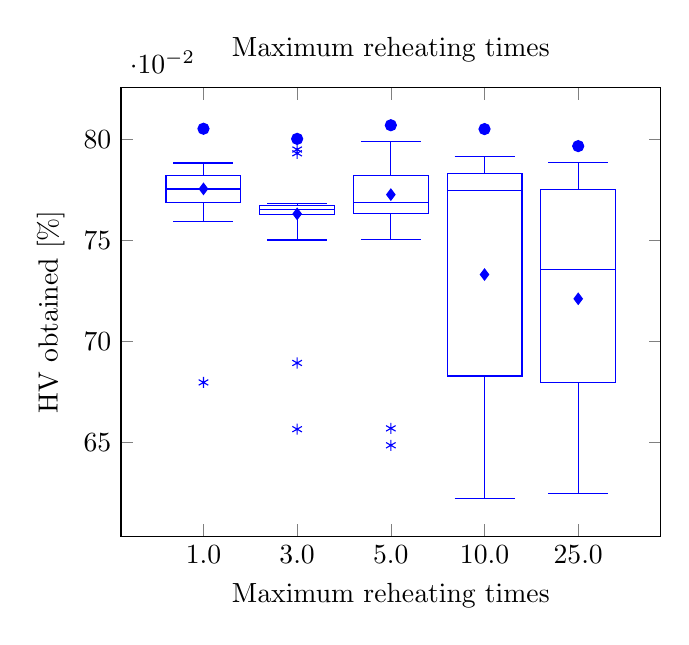
\begin{tikzpicture} 
\begin{axis}[ 
title={Maximum reheating times}, 
boxplot/draw direction=y, 
xtick={1,2,3,4,5}, 
xticklabels={1.0,3.0,5.0,10.0,25.0}, 
x tick label style={rotate=0, align=center}, 
xlabel={Maximum reheating times}, 
% y tick label style={/pgf/number format/.cd,fixed,precision=3, zerofill}, 
scaled y ticks={base 10:2}, 
ylabel={HV obtained [\%]}, 
] 

% ############## max_reheating_times=1.0 ################## 
\addplot[boxplot, mark=asterisk, 
boxplot prepared={ 
lower whisker=0.75938, 
upper whisker=0.78847, 
lower quartile=0.7687, 
upper quartile=0.78249, 
median=0.77558, 
average=0.77564}, 
color = blue, solid, area legend] 
coordinates {
(1,0.67975)}; 
\addplot[only marks,mark=*,color = blue]coordinates{(1,0.80545)}; 

% ############## max_reheating_times=3.0 ################## 
\addplot[boxplot, mark=asterisk, 
boxplot prepared={ 
lower whisker=0.75035, 
upper whisker=0.76832, 
lower quartile=0.76294, 
upper quartile=0.76755, 
median=0.76524, 
average=0.76327}, 
color = blue, solid, area legend] 
coordinates {
(2,0.68939)
(2,0.65659)
(2,0.79516)
(2,0.79329)}; 
\addplot[only marks,mark=*,color = blue]coordinates{(2,0.80044)}; 

% ############## max_reheating_times=5.0 ################## 
\addplot[boxplot, mark=asterisk, 
boxplot prepared={ 
lower whisker=0.75049, 
upper whisker=0.79917, 
lower quartile=0.76357, 
upper quartile=0.78238, 
median=0.7691, 
average=0.7728}, 
color = blue, solid, area legend] 
coordinates {
(3,0.64861)
(3,0.65699)}; 
\addplot[only marks,mark=*,color = blue]coordinates{(3,0.80719)}; 

% ############## max_reheating_times=10.0 ################## 
\addplot[boxplot, mark=asterisk, 
boxplot prepared={ 
lower whisker=0.62208, 
upper whisker=0.79153, 
lower quartile=0.68295, 
upper quartile=0.78326, 
median=0.77466, 
average=0.7332}, 
color = blue, solid, area legend] 
coordinates {}; 
\addplot[only marks,mark=*,color = blue]coordinates{(4,0.80529)}; 

% ############## max_reheating_times=25.0 ################## 
\addplot[boxplot, mark=asterisk, 
boxplot prepared={ 
lower whisker=0.62461, 
upper whisker=0.78877, 
lower quartile=0.6796, 
upper quartile=0.77555, 
median=0.73564, 
average=0.7212}, 
color = blue, solid, area legend] 
coordinates {}; 
\addplot[only marks,mark=*,color = blue]coordinates{(5,0.79685)}; 

\end{axis}
\end{tikzpicture}
\end{figure} 

% ######################## UTRP SA Minimum accepts ######################## 
\begin{figure} 
\centering 
\tikzsetnextfilename{UTRP_DBMOSA_BP_min_accepts} 
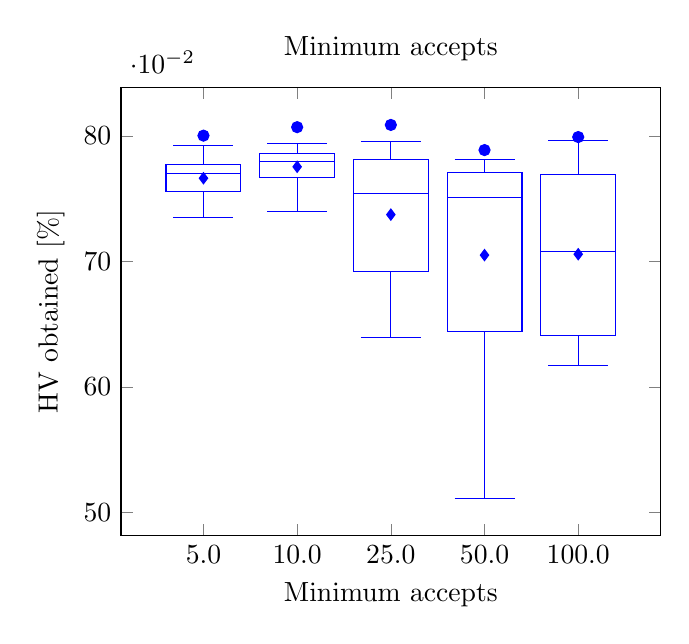
\begin{tikzpicture} 
\begin{axis}[ 
title={Minimum accepts}, 
boxplot/draw direction=y, 
xtick={1,2,3,4,5}, 
xticklabels={5.0,10.0,25.0,50.0,100.0}, 
x tick label style={rotate=0, align=center}, 
xlabel={Minimum accepts}, 
% y tick label style={/pgf/number format/.cd,fixed,precision=3, zerofill}, 
scaled y ticks={base 10:2}, 
ylabel={HV obtained [\%]}, 
] 

% ############## min_accepts=5.0 ################## 
\addplot[boxplot, mark=asterisk, 
boxplot prepared={ 
lower whisker=0.73497, 
upper whisker=0.79211, 
lower quartile=0.7556, 
upper quartile=0.7775, 
median=0.77023, 
average=0.76625}, 
color = blue, solid, area legend] 
coordinates {}; 
\addplot[only marks,mark=*,color = blue]coordinates{(1,0.8002)}; 

% ############## min_accepts=10.0 ################## 
\addplot[boxplot, mark=asterisk, 
boxplot prepared={ 
lower whisker=0.73992, 
upper whisker=0.79422, 
lower quartile=0.76708, 
upper quartile=0.78627, 
median=0.77932, 
average=0.77539}, 
color = blue, solid, area legend] 
coordinates {}; 
\addplot[only marks,mark=*,color = blue]coordinates{(2,0.80695)}; 

% ############## min_accepts=25.0 ################## 
\addplot[boxplot, mark=asterisk, 
boxplot prepared={ 
lower whisker=0.63954, 
upper whisker=0.79563, 
lower quartile=0.69197, 
upper quartile=0.78142, 
median=0.7543, 
average=0.73726}, 
color = blue, solid, area legend] 
coordinates {}; 
\addplot[only marks,mark=*,color = blue]coordinates{(3,0.80873)}; 

% ############## min_accepts=50.0 ################## 
\addplot[boxplot, mark=asterisk, 
boxplot prepared={ 
lower whisker=0.51102, 
upper whisker=0.78128, 
lower quartile=0.64422, 
upper quartile=0.77076, 
median=0.7508, 
average=0.70501}, 
color = blue, solid, area legend] 
coordinates {}; 
\addplot[only marks,mark=*,color = blue]coordinates{(4,0.7887)}; 

% ############## min_accepts=100.0 ################## 
\addplot[boxplot, mark=asterisk, 
boxplot prepared={ 
lower whisker=0.61705, 
upper whisker=0.79622, 
lower quartile=0.64077, 
upper quartile=0.76931, 
median=0.70773, 
average=0.7057}, 
color = blue, solid, area legend] 
coordinates {}; 
\addplot[only marks,mark=*,color = blue]coordinates{(5,0.79907)}; 

\end{axis}
\end{tikzpicture}
\end{figure} 

% ######################## UTRP SA Reheating rate ######################## 
\begin{figure} 
\centering 
\tikzsetnextfilename{UTRP_DBMOSA_BP_reheating_rate} 
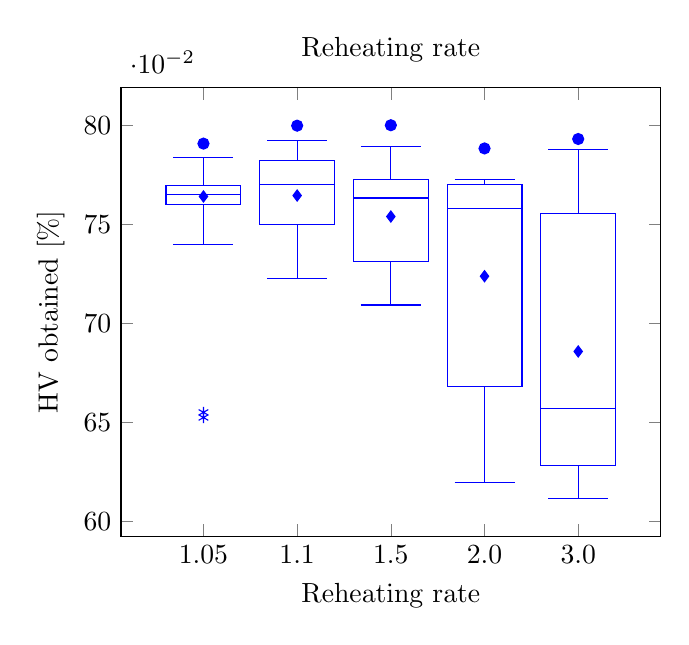
\begin{tikzpicture} 
\begin{axis}[ 
title={Reheating rate}, 
boxplot/draw direction=y, 
xtick={1,2,3,4,5}, 
xticklabels={1.05,1.1,1.5,2.0,3.0}, 
x tick label style={rotate=0, align=center}, 
xlabel={Reheating rate}, 
% y tick label style={/pgf/number format/.cd,fixed,precision=3, zerofill}, 
scaled y ticks={base 10:2}, 
ylabel={HV obtained [\%]}, 
] 

% ############## Reheating_rate=1.05 ################## 
\addplot[boxplot, mark=asterisk, 
boxplot prepared={ 
lower whisker=0.73991, 
upper whisker=0.78393, 
lower quartile=0.76, 
upper quartile=0.76976, 
median=0.76539, 
average=0.76421}, 
color = blue, solid, area legend] 
coordinates {
(1,0.65504)
(1,0.65241)}; 
\addplot[only marks,mark=*,color = blue]coordinates{(1,0.79093)}; 

% ############## Reheating_rate=1.1 ################## 
\addplot[boxplot, mark=asterisk, 
boxplot prepared={ 
lower whisker=0.72282, 
upper whisker=0.79258, 
lower quartile=0.75014, 
upper quartile=0.78261, 
median=0.7703, 
average=0.76467}, 
color = blue, solid, area legend] 
coordinates {}; 
\addplot[only marks,mark=*,color = blue]coordinates{(2,0.8)}; 

% ############## Reheating_rate=1.5 ################## 
\addplot[boxplot, mark=asterisk, 
boxplot prepared={ 
lower whisker=0.70934, 
upper whisker=0.7896, 
lower quartile=0.73145, 
upper quartile=0.77291, 
median=0.76343, 
average=0.75403}, 
color = blue, solid, area legend] 
coordinates {}; 
\addplot[only marks,mark=*,color = blue]coordinates{(3,0.80022)}; 

% ############## Reheating_rate=2.0 ################## 
\addplot[boxplot, mark=asterisk, 
boxplot prepared={ 
lower whisker=0.6195, 
upper whisker=0.77256, 
lower quartile=0.6682, 
upper quartile=0.77033, 
median=0.75791, 
average=0.72388}, 
color = blue, solid, area legend] 
coordinates {}; 
\addplot[only marks,mark=*,color = blue]coordinates{(4,0.78849)}; 

% ############## Reheating_rate=3.0 ################## 
\addplot[boxplot, mark=asterisk, 
boxplot prepared={ 
lower whisker=0.6113, 
upper whisker=0.78792, 
lower quartile=0.62815, 
upper quartile=0.75544, 
median=0.65717, 
average=0.68582}, 
color = blue, solid, area legend] 
coordinates {}; 
\addplot[only marks,mark=*,color = blue]coordinates{(5,0.79326)}; 

\end{axis}
\end{tikzpicture}
\end{figure} 

% ######################## UTRP SA Starting temperature ######################## 
\begin{figure} 
\centering 
\tikzsetnextfilename{UTRP_DBMOSA_BP_initial_temp} 
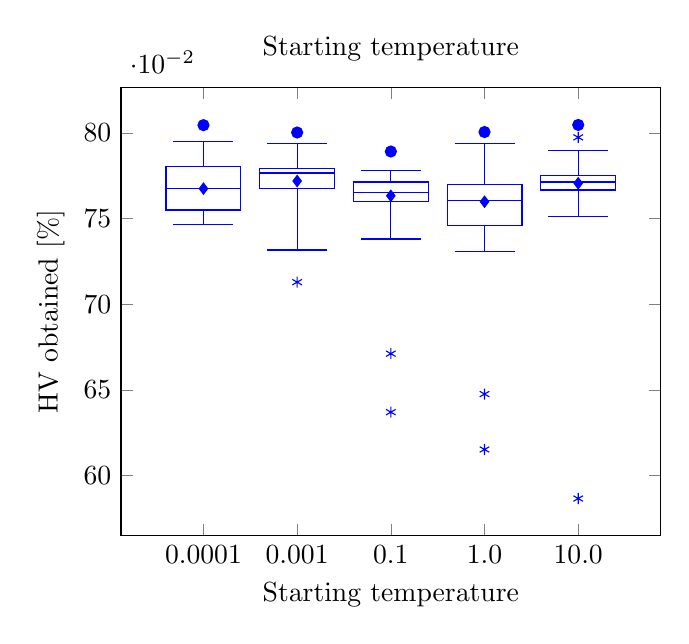
\begin{tikzpicture} 
\begin{axis}[ 
title={Starting temperature}, 
boxplot/draw direction=y, 
xtick={1,2,3,4,5}, 
xticklabels={0.0001,0.001,0.1,1.0,10.0}, 
x tick label style={rotate=0, align=center}, 
xlabel={Starting temperature}, 
% y tick label style={/pgf/number format/.cd,fixed,precision=3, zerofill}, 
scaled y ticks={base 10:2}, 
ylabel={HV obtained [\%]}, 
] 

% ############## Temp=0.0001 ################## 
\addplot[boxplot, mark=asterisk, 
boxplot prepared={ 
lower whisker=0.74675, 
upper whisker=0.79472, 
lower quartile=0.75498, 
upper quartile=0.78041, 
median=0.76734, 
average=0.76746}, 
color = blue, solid, area legend] 
coordinates {}; 
\addplot[only marks,mark=*,color = blue]coordinates{(1,0.80448)}; 

% ############## Temp=0.001 ################## 
\addplot[boxplot, mark=asterisk, 
boxplot prepared={ 
lower whisker=0.73164, 
upper whisker=0.79376, 
lower quartile=0.76727, 
upper quartile=0.77943, 
median=0.77654, 
average=0.77187}, 
color = blue, solid, area legend] 
coordinates {
(2,0.7129)}; 
\addplot[only marks,mark=*,color = blue]coordinates{(2,0.80019)}; 

% ############## Temp=0.1 ################## 
\addplot[boxplot, mark=asterisk, 
boxplot prepared={ 
lower whisker=0.73809, 
upper whisker=0.77822, 
lower quartile=0.75984, 
upper quartile=0.77131, 
median=0.76511, 
average=0.76326}, 
color = blue, solid, area legend] 
coordinates {
(3,0.67119)
(3,0.63707)}; 
\addplot[only marks,mark=*,color = blue]coordinates{(3,0.78911)}; 

% ############## Temp=1.0 ################## 
\addplot[boxplot, mark=asterisk, 
boxplot prepared={ 
lower whisker=0.73093, 
upper whisker=0.79381, 
lower quartile=0.74611, 
upper quartile=0.77012, 
median=0.76035, 
average=0.75981}, 
color = blue, solid, area legend] 
coordinates {
(4,0.64763)
(4,0.61531)}; 
\addplot[only marks,mark=*,color = blue]coordinates{(4,0.80046)}; 

% ############## Temp=10.0 ################## 
\addplot[boxplot, mark=asterisk, 
boxplot prepared={ 
lower whisker=0.75128, 
upper whisker=0.78954, 
lower quartile=0.76664, 
upper quartile=0.77529, 
median=0.77133, 
average=0.77059}, 
color = blue, solid, area legend] 
coordinates {
(5,0.79735)
(5,0.5867)}; 
\addplot[only marks,mark=*,color = blue]coordinates{(5,0.80461)}; 

\end{axis}
\end{tikzpicture}
\end{figure} 
\begin{table}
\centering
\caption{Legend for the boxplot.}
\begin{tabular}{ll}
\toprule
 Index &  Name \\
\midrule
     0 &    10 \\
     1 &    50 \\
     2 &   100 \\
     3 &   250 \\
     4 &   500 \\
\bottomrule
\end{tabular}
\end{table}

\end{document}
